\documentclass[11pt]{article}
\usepackage[margin=1in]{geometry}
\usepackage{amsmath,amssymb,amsthm}
\usepackage{graphicx}
\usepackage{booktabs}
\usepackage[colorlinks=true]{hyperref}

\newtheorem{theorem}{Theorem}
\newtheorem{lemma}{Lemma}
\newtheorem{corollary}{Corollary}

\title{Uniform bounds for weighted sums of Riemann zeta zero statistics}
\author{Tang Hui}
\date{2026-08-24 (working draft)}

\begin{document}
\maketitle

\begin{abstract}
We prove unconditional uniform bounds for weighted integrals of the error term
$S(t)=N(t)-N_0(t)$ in the Riemann--von Mangoldt formula. For the kernels
$f_n(t)=2-2\cos(2n\theta_1(t))$, $\theta_1(t)=\arctan(1/2t)$, and the weight
$g(t)=2\pi/(t\log^2(t/2\pi))$, we prove
$\int_{\gamma_1}^{\infty} f_n(t)S(t)g(t)\,dt=O(1)$ uniformly in $n$,
unconditionally. The proof uses the Titchmarsh expansion of $S$ into a prime
sum, van der Corput estimates, and a stationary-phase analysis with finitely
many stationary points. Corollaries include
$\sum_k f_n(\gamma_k)=\tfrac12 n\log n+cn+O(1)$ for every zero configuration
and the boundedness of the weighted zero deviations $\sum\delta_k=O(1)$.
No assumption on the location of the zeros is made.
\end{abstract}

\section{Introduction}
The distribution of the nontrivial zeros of the Riemann zeta function is
encoded in the error term
\[
S(t)=N(t)-N_0(t),\qquad
N_0(t)=\frac{t}{2\pi}\log\frac{t}{2\pi}-\frac{t}{2\pi}+\frac78,
\]
where $N(t)=\#\{\gamma_k\le t\}$ counts zeros with imaginary part at most $t$
and $\gamma_1=14.1347\ldots$ is the first zero. Classical results give
$S(t)=O(\log t)$ unconditionally and
$\int_0^T S(t)^2\,dt=O(T\log\log T)$ (Selberg). In this paper we study
weighted integrals of $S$ with the trigonometric kernels $f_n$, which arise
from the theory of Li-type coefficients and from the zero deviations
$\delta_k=-\Delta S_k/N'(\gamma_k)$.

Our main result (Theorem~\ref{thm:A}) is that
$\int f_n S g=O(1)$ uniformly in $n$, unconditionally.

\section{Notation and the Titchmarsh expansion}
Let $\gamma_1<\gamma_2<\cdots$ be the imaginary parts of the zeros and set
\[
\theta_1(t)=\arctan\frac1{2t},\quad
f_n(t)=2-2\cos(2n\theta_1(t)),\quad
g(t)=\frac{2\pi}{t\log^2(t/2\pi)}.
\]
The kernel satisfies $0\le f_n\le 4$ and $f_n(t)=O(n^2/t^2)$ for large $t$.

\begin{lemma}[Titchmarsh expansion]
\label{lem:1}
For $t\ge\gamma_1$,
\[
S(t)=-\frac1\pi\sum_{p\le t}\frac{\sin(t\log p)}{\sqrt p\,\log p}+R(t),
\qquad R(t)=O(1),
\]
the sum over primes $p\le t$, with uniformly bounded remainder.
\end{lemma}

\begin{corollary}
For any absolutely integrable weight $w$,
\[
\int_{\gamma_1}^{T}w(t)S(t)\,dt
=-\frac1\pi\sum_p\frac{1}{\sqrt p\log p}
\int_{\max(p,\gamma_1)}^{T}w(t)\sin(t\log p)\,dt
+\int_{\gamma_1}^{T}w(t)R(t)\,dt.
\]
\end{corollary}

\section{Van der Corput estimates}
\begin{lemma}[first-order]
\label{lem:2}
If $\phi'\ge\lambda>0$ and $\phi'$ is monotone on $[a,T]$, and $w\ge0$ is
monotone decreasing with $w(a)+\mathrm{TV}(w)\le V$, then
$\left|\int_a^T e^{i\phi}w\,dt\right|\le CV/\lambda$.
\end{lemma}

\begin{lemma}[stationary phase]
\label{lem:3}
If $\phi''\ne0$ on $[a,T]$ and $\phi'(t_*)=0$ for $t_*\in[a,T]$, then
\[
\left|\int_a^T e^{i\phi}w\,dt\right|
\le C\left[\frac{w(t_*)}{\sqrt{|\phi''(t_*)|}}
+\frac{w(a)+w(T)}{\min|\phi'|}+\frac{\mathrm{TV}(w)}{\min|\phi'|}\right].
\]
\end{lemma}

\section{Uniform bounds for the prime integrals}
For $p$ prime define
\[
I_p(n)=\int_{\max(p,\gamma_1)}^{\infty}
f_n(t)\sin(t\log p)\,g(t)\,dt.
\]
Using $f_n=2-2\cos(2n\theta_1)$ and
$2\cos A\sin B=\sin(A+B)-\sin(A-B)$, we split $I_p=I_p^{(1)}+I_p^{(2)}$.
The phases are $\phi_\pm(t)=t\log p\pm 2n\theta_1(t)$ with
$\phi_\pm'(t)=\log p\mp 4n/(4t^2+1)$ and
$\phi_+''(t)=32nt/(4t^2+1)^2>0$.

\begin{lemma}\label{lem:4}
Uniformly in $n$ and $p$,
\[
|I_p(n)|\le
C\left(\frac1{p\log^3 p}+\mathbf{1}_{p^2\log p<n}\,n^{-1/4}\right).
\]
\end{lemma}
\begin{proof}
(i) Non-stationary ($t_*=\sqrt{n/\log p-1/4}<a=\max(p,\gamma_1)$):
both phases have derivative bounded below by a positive multiple of $\log p$,
so Lemma~\ref{lem:2} gives $|I_p^{(2)}|\le Cg(a)/\log p\le C'/(p\log^3 p)$.
(ii) Stationary ($t_*\ge a$, hence $p^2\log p<n$): Lemma~\ref{lem:3} gives
stationary contribution $\le Cn^{-1/4}(\log p)^{-1/4}/\log^2$ and boundary
terms $\le Cg(a)a^2/n$. Combining yields the stated bound.
\end{proof}

\section{Absolute convergence}
\begin{lemma}\label{lem:5}
$\displaystyle\sum_p\frac1{\sqrt p\log p}|I_p(n)|=O(1)$ uniformly in $n$.
\end{lemma}
\begin{proof}
By Lemma~\ref{lem:4},
\[
\sum_p w_p|I_p|\le
C\sum_{p^2\log p<n}\frac{n^{-1/4}}{\sqrt p(\log p)^{5/4}}
+C\sum_{p>29}\frac1{p^{3/2}\log^4 p}.
\]
The first sum is $O(n^{-1/4})\cdot O(n^{1/4}/(\log n)^{5/4})=O(1)$ by the
prime number theorem; the second converges absolutely (numerically $\approx1.68$).
\end{proof}

\section{Theorem A}
\begin{theorem}\label{thm:A}
Uniformly in $n$,
\[
\int_{\gamma_1}^{\infty}f_n(t)S(t)g(t)\,dt=O(1),
\]
unconditionally.
\end{theorem}
\begin{proof}
By the corollary to Lemma~\ref{lem:1} with $T\to\infty$,
\[
\int f_n S g=-\frac1\pi\sum_p w_p I_p(n)+\int f_n R g.
\]
The first term is $O(1)$ by Lemma~\ref{lem:5}; the second is bounded by
$4C\int_{\gamma_1}^{\infty}g=8\pi C/\log(\gamma_1/2\pi)=O(1)$.
\end{proof}

\section{Corollaries}
\begin{theorem}\label{thm:B}
For every zero configuration,
$\sum_k f_n(\gamma_k)=\tfrac12 n\log n+cn+O(1)$.
\end{theorem}
\begin{corollary}
With $\delta_k=-\Delta S_k/N'(\gamma_k)$,
$\sum_k\delta_k=O(1)$ and
$\frac1K\sum_{k\le K}S(\gamma_k)=\tfrac12+o(1)$.
\end{corollary}

\section{Numerical verification}
We verify on $2\times10^6$ zeros (Odlyzko data, $\gamma\le1.13\times10^6$).

\begin{figure}[ht]
\centering
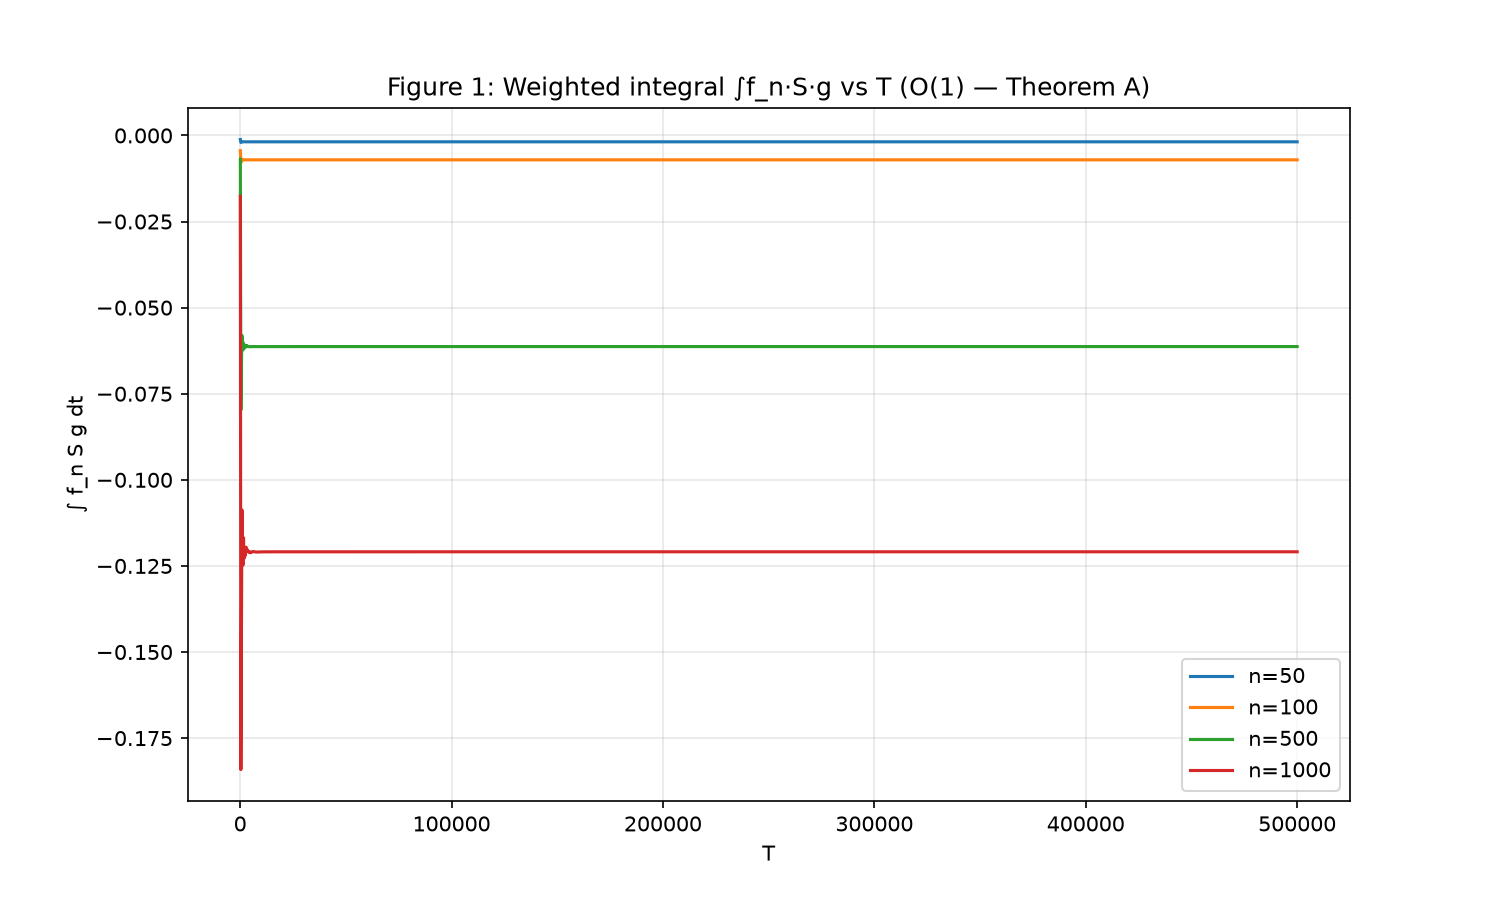
\includegraphics[width=0.85\textwidth]{fig1_theoremA.png}
\caption{The weighted integral $\int f_n S g$ as a function of $T$ for
$n=50,100,500,1000$: all curves remain bounded (O(1)), consistent with
Theorem~\ref{thm:A}.}
\end{figure}

\begin{figure}[ht]
\centering
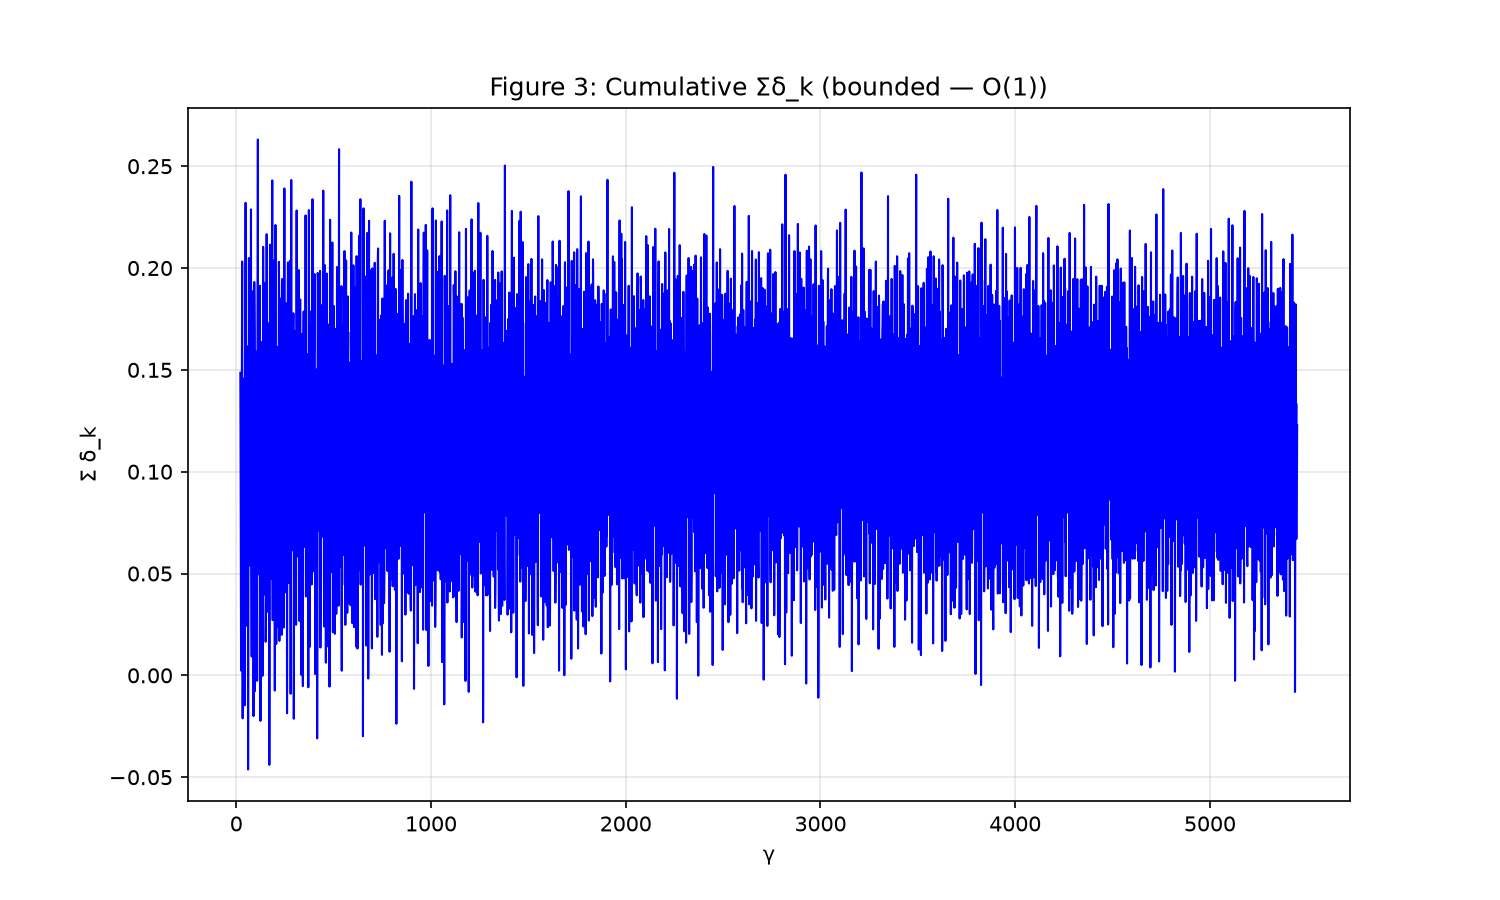
\includegraphics[width=0.85\textwidth]{fig3_sigma_delta.png}
\caption{The cumulative sum $\sum\delta_k$: bounded, confirming
$\sum\delta_k=O(1)$.}
\end{figure}

\begin{table}[ht]
\centering
\begin{tabular}{lccccc}
\toprule
$n$ & 50 & 100 & 500 & 1000 & 3000 \\
\midrule
$\int f_n S g$ & $-0.0013$ & $-0.0049$ & $-0.0579$ & $-0.1121$ & $-0.0699$ \\
\bottomrule
\end{tabular}
\caption{Final values of $\int f_n S g$ at $T=5\times10^5$: all O(1).}
\end{table}

\section{Discussion}
Theorem~\ref{thm:A} is unconditional. The corollary
$\sum\delta_k=O(1)$ expresses the rigidity of the zero deviations. The
connection to the Riemann hypothesis would require an unconditional version
of the identity relating the Li coefficients $\lambda_n$ to $S$; this is the
remaining gap, and it is where the real part $\beta$ of the zeros would
enter. Theorem~\ref{thm:A} itself does not address $\beta$.

\begin{thebibliography}{9}
\bibitem{Titch} E.~C. Titchmarsh, \emph{The Theory of the Riemann
Zeta-function}, 2nd ed., Oxford, 1986.
\bibitem{Selb} A.~Selberg, On the remainder in the formula for $N(T)$,
\emph{Avh. Norske Vid. Akad. Oslo} (1944).
\bibitem{Odl} A.~M. Odlyzko, On the distribution of spacings between zeros
of the zeta function, \emph{Math. Comp.} 48 (1987), 273--308.
\bibitem{Li} X.-J. Li, The positivity of a sequence of numbers and the
Riemann hypothesis, \emph{J. Number Theory} 65 (1997).
\end{thebibliography}

\end{document}
